% IncludeFile style
% Typical usage (all UPPERCASE items are optional):
%       \input includeFile
%       \begin{document}
%       \MYTITLE{Title of document, e.g., Lab 1\\Due ...}
%       \MYHEADERS{short title}{other running head, e.g., due date}
%       \PURPOSE{Description of purpose}
%       \SUMMARY{Very short overview of assignment}
%       \DETAILS{Detailed description}
%         \SUBHEAD{if needed} ...
%         \SUBHEAD{if needed} ...
%          ...
%       \HANDIN{What to hand in and how}
%       \begin{checklist}
%       \item ...
%       \end{checklist}
% There is no need to include a "\documentstyle."
% However, there should be an "\end{document}."
%
%===========================================================
\documentclass[11pt,twoside,titlepage]{article}
%%NEED TO ADD epsf!!
\usepackage{threeparttop}
\usepackage{graphicx}
\usepackage{latexsym}
\usepackage{color}
\usepackage{listings}
\usepackage{fancyvrb}
%\usepackage{pgf,pgfarrows,pgfnodes,pgfautomata,pgfheaps,pgfshade}
\usepackage{tikz}
\usepackage[normalem]{ulem}
\tikzset{
    %Define standard arrow tip
%    >=stealth',
    %Define style for boxes
    oval/.style={
           rectangle,
           rounded corners,
           draw=black, very thick,
           text width=6.5em,
           minimum height=2em,
           text centered},
    % Define arrow style
    arr/.style={
           ->,
           thick,
           shorten <=2pt,
           shorten >=2pt,}
}
\usepackage[noend]{algorithmic}
\usepackage[noend]{algorithm}
\newcommand{\bfor}{{\bf for\ }}
\newcommand{\bthen}{{\bf then\ }}
\newcommand{\bwhile}{{\bf while\ }}
\newcommand{\btrue}{{\bf true\ }}
\newcommand{\bfalse}{{\bf false\ }}
\newcommand{\bto}{{\bf to\ }}
\newcommand{\bdo}{{\bf do\ }}
\newcommand{\bif}{{\bf if\ }}
\newcommand{\belse}{{\bf else\ }}
\newcommand{\band}{{\bf and\ }}
\newcommand{\breturn}{{\bf return\ }}
\newcommand{\mod}{{\rm mod}}
\renewcommand{\algorithmiccomment}[1]{$\rhd$ #1}
\newenvironment{checklist}{\par\noindent\hspace{-.25in}{\bf Checklist:}\renewcommand{\labelitemi}{$\Box$}%
\begin{itemize}}{\end{itemize}}
\pagestyle{threepartheadings}
\usepackage{url}
\usepackage{wrapfig}
% removing the standard hyperref to avoid the horrible boxes
%\usepackage{hyperref}
\usepackage[hidelinks]{hyperref}
% added in the dtklogos for the bibtex formatting
%\usepackage{dtklogos}
%=========================
% One-inch margins everywhere
%=========================
\setlength{\topmargin}{0in}
\setlength{\textheight}{8.5in}
\setlength{\oddsidemargin}{0in}
\setlength{\evensidemargin}{0in}
\setlength{\textwidth}{6.5in}
%===============================
%===============================
% Macro for document title:
%===============================
\newcommand{\MYTITLE}[1]%
   {\begin{center}
     \begin{center}
     \bf
     CMPSC 300\\Bioinformatics\\
     Fall 2019 
     \medskip
     \end{center}
     \bf
     #1
     \end{center}
}
%================================
% Macro for headings:
%================================
\newcommand{\MYHEADERS}[3]%
   {\lhead{#1}
    \rhead{#2}

%    \def \dateofhandout {January 17, 2017}
%    \lfoot{\sc Handed out on \dateofhandout}

    \def \dateofhandout {#3}
    \lfoot{\sc \dateofhandout}

   }

%================================
% Macro for bold italic:
%================================
\newcommand{\bit}[1]{{\textit{\textbf{#1}}}}

%=========================
% Non-zero paragraph skips.
%=========================
\setlength{\parskip}{1ex}

%=========================
% Create various environments:
%=========================
\newcommand{\PURPOSE}{\par\noindent\hspace{-.25in}{\bf Purpose:\ }}
\newcommand{\SUMMARY}{\par\noindent\hspace{-.25in}{\bf Summary:\ }}
\newcommand{\DETAILS}{\par\noindent\hspace{-.25in}{\bf Details:\ }}
\newcommand{\HANDIN}{\par\noindent\hspace{-.25in}{\bf Hand in:\ }}
\newcommand{\SUBHEAD}[1]{\bigskip\par\noindent\hspace{-.1in}{\sc #1}\\}
%\newenvironment{CHECKLIST}{\begin{itemize}}{\end{itemize}}



\long\def\omitit #1{}

\begin{document}


\MYTITLE{Lab 2:\\ DNA and Python3 Basics}
\MYHEADERS{}{\color{red} Due: 16$^{th}$ Sept\color{black}}{Handed out: 9$^{th}$ Sept. 2019}
% Due: 9$^{th}$ Sept
\flushleft

%\MYTITLE{Lab 2: Laboratory Assignment Two: DNA and Python Basics. \\ \color{red}Save this lab assignment to: {\tt labs/lab2}\color{black}}
%\MYHEADERS{Introduction to Bioinformatics}{Due: 13 Sept.}{Handed out on: 6 Sept. 2017}

\begin{figure}[ht!]
	\begin{center}
	 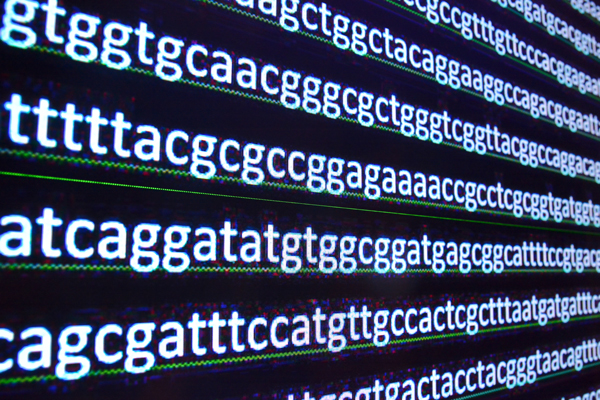
\includegraphics[scale=.3]{graphics/writtenDNA.jpg}
	\end{center}
\end{figure}


\subsection*{Summary}

To strengthen the understanding of DNA structure and DNA replication. To learn and enhance your Python3 programming skills, including how to create variables, write assignment statements, manipulate lists, create repetitive and conditional statements. To utilize basic Python programming skills to write a program that processes and manipulates the DNA sequence.



\subsubsection*{GitHub starter link}
\begin{center}
\color{red} \url{https://classroom.github.com/a/ntDDrfDl} \color{black}
\end{center}



To use this link, please follow the steps below.
\begin{itemize}
	\item Click on the link and accept the assignment.
	\item Once the importing task has completed, click on the created assignment link which will take you to your newly created GitHub repository for this lab.
	\item Clone this repository (bearing your name) and work on the practical locally.
	\item As you are working on your practical, you are to commit and push regularly. You can use the following commands to add a single file, you must be in the directory where the file is located (or add the path to the file in the command):
		\begin{itemize}
		\item {\tt git add -A}
		\item {\tt git commit -m ``Your notes about commit here''}
		\item {\tt git push}
	\end{itemize}

	Alternatively, you can use the following commands to add multiple files from your repository:
	\begin{itemize}
		\item {\tt git commit <}\emph{nameOfFile}\tt{> -m ``Your notes about commit here''}
		\item {\tt git push}
	\end{itemize}
\end{itemize}
%%%

Be sure to read the {\tt README.md} file in the GitHub Classroom repository for instructions on how to complete your first assignment.


\section*{DNA and Python Basics}

Bioinformatics requires the use of computational techniques to solve biologically-related problems. Therefore, in this course it is essential for you to have some basic understanding of both biological 
and computer science concepts related to Bioinformatics before we approach Bioinformatics problems. 

Seemingly all goals of Bioinformatics research depend on automation for completion. In many cases, bioinformaticians are required to create their own programs and tools in order to complete their cutting-edge work. In this lab, you will also create a basic tool to help in your future work in the field. 

%As we discuss the foundational background material from Biology and computer programming in class in the next two weeks, during the next two lab sessions you will be invited to strengthen your biological understanding and have more hands-on experience with basic programming in Python. 


\vspace*{-.1in}
\section*{Part 1: DNA Structure Worksheet}
\vspace*{-.1in} 
Navigate to the activity your GitHub Classroom repository (\color{red}{\tt activity/activitySheet.md}\color{black}). Please complete the assignment by writing in your responses in markdown formatting into the file.



\vspace*{-.1in}
\section*{Part 2: Getting to Know Python}
\vspace*{-.1in} 

\subsection*{Python Help}
Before we can start writing Python programs for Bioinformatics solutions, you need to get comfortable with the structure and the syntax of this programming language. Just like with any natural or programming language, you need to learn various syntactical and semantic rules when writing in Python.

If you feel that your skill in Python3 needs some improvement, you are invited to read Chapters 1 and 2 in the ``Think Python'' textbook. To get started with Python, please complete Sections 3 and 4.1-4.5 in the Python Tutorial, which can be found in: \url{https://docs.python.org/3/tutorial/index.html}. NOTE: if you have a previous experience in using Python, please browse through the tutorial and then consider lending your expertise to your fellow classmate.

\noindent Now that you have been exposed to some basic rules of programming in Python, you are asked to practice those skills by writing  programs to accomplish the following small tasks.


\vspace*{-.1in}
\subsection*{Python3 Coding: a DNA Base Counting Program}
\vspace*{-.1in} 
%DNA (deoxyribonucleic acid) is the building block of every organism. It contains information about hair color, skin tone, allergies, and more.  DNA is composed of four bases - adenine, thymine, cytosine, guanine. A string is simply an ordered collection of symbols selected from some alphabet and formed into a word with the length of a string being the number of symbols that it contains. An example of a length 21 DNA string (whose alphabet contains the symbols `A', `C', `G', and `T') is ``ATGCTTCAGAAAGGTCTTACG.'' 

You are to write a Python program that:

\noindent \textbf{Given}: A DNA string of length at most 1000 nt. \\ 
\textbf{Returns}: Four integers (separated by spaces) counting the respective number of times that the bases,`A', `C', `G', and `T' occur in the sequence. In addition, you are to add the pair-counts of ``AT'', ``TA''. ``GC'' and ``CG''. Your programming is to simply go though the string and count these combinations. 

\emph{Sample Input: } \\
AAAACCCGGT \\

\emph{Sample Output: } \\
	\begin{itemize}
	
	\item A's: 4 
  	\item C's: 3
  	\item G's: 2
  	\item T's: 1
\end{itemize}

\noindent
Note: your source file is to be called: {\tt \color{red} baseCounter.py\color{black}}



%%%%%%%%%%%%%%%%%%%%%%%%%%%%

\vspace*{-.1in}
\subsection*{Python3 Coding: Find the Complementary sequence of DNA}
\vspace*{-.1in} 
DNA's bases are paired as follows: A$\leftrightarrow $T and G$\leftrightarrow $C. 

You are to write a Python program that:

\noindent \textbf{Given}: A DNA string of length at most 1000 nt. \\ 
\textbf{Returns}: The complementary base string of the entered DNA. 

\emph{Sample Input: } \\
AAAACCCGGT \\

\emph{Sample Output:}\\
	\begin{itemize}
		\item TTTTGGGCCA
	\end{itemize}



Note: your source file is to be called: {\color{red}\tt compSeq.py \color{black}}
%%%%%%%%%%%%%%%






\subsection*{Ethical Portion}

Locate the article in your repository by Michael Specter entitled, "Rewriting the code of life." (The New Yorker, 2017.

The reference to the article is \url{https://www.newyorker.com/magazine/2017/01/02/rewriting-the-code-of-life?reload=true}

Please complete the three questions found in the file, {\tt \color{red} ethics/reflections.md \color{black}}




\vspace*{-.2in}
\subsection*{Required Deliverables}
\vspace*{-.1in}

\begin{itemize}
	\item Your completed activity should be saved as {\tt \color{red} activity/activitySheet.md\color{black}.}


	\item All of the deliverables (i.e., {\tt baseCounter.py} and {\tt comp.py}) of Part 2 are to be placed into your {\tt src} folder in your GitHub Classroom repository. Please ensure that you have sent your files correctly to the GitHub correctly by visiting the web site of your repository and by checking the your source files. This will show you whether you have correctly pushed your files. Please ask questions, if necessary.
    \item The ethical reflections writing piece: {\tt \color{red} ethics/reflections.md \color{black}.
	
	\end{itemize}

\noindent You should see the instructor if you have questions about assignment submission.
\end{document}




